\documentclass{article}
\usepackage[T1]{fontenc}
\usepackage{lmodern}
\usepackage{graphicx}
\usepackage{amsmath,amssymb}
\usepackage[a4paper,margin=2cm]{geometry}
\usepackage[absolute,overlay]{textpos}
\setlength{\TPHorizModule}{1mm}
\setlength{\TPVertModule}{1mm}
\usepackage[indonesian]{babel}
\usepackage{hyperref}
\setlength{\emergencystretch}{2em}
% unit: Halaman 66

\begin{document}

% === Halaman 66 (python/native) ===

66

C. Playfair Cipher 

• Ditemukan oleh Sir Charles Wheatstone namun dipromosikan oleh 

Baron Lyon Playfair pada tahun 1854.

The Playfair system was invented by Charles Wheatstone, who first described it in 1854.

Lord Playfair promoted the use of the cipher, and his name became associated with the system.

Sir Charles Wheatstone

Baron Lyon Playfair

% deskripsi: gambar native xref 250
\noindent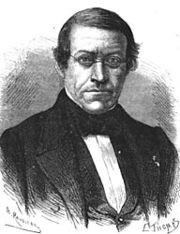
\includegraphics[width=0.85\textwidth]{../../images/python/page_066_img_01.jpeg}

% deskripsi: gambar native xref 252
\noindent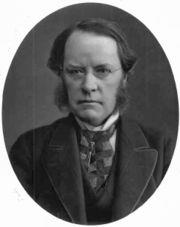
\includegraphics[width=0.85\textwidth]{../../images/python/page_066_img_02.jpeg}

\end{document}
